\pdfoutput=1
\documentclass[letterpaper]{article}
\usepackage{times}
\usepackage{graphicx}
\usepackage{appendix}
\usepackage{amsmath}
\usepackage{float}
\usepackage{tikz,pgfplots}
\pgfplotsset{width=6cm}
\usepackage[superscript]{cite}
\usepackage{hyperref}
\usepackage[toc]{glossaries}

\usetikzlibrary{decorations.pathreplacing}
\usepackage{algorithm,algorithmic,a4wide,amssymb,natbib,multicol,enumitem,url}
\usepackage[top=3cm, bottom=3cm, left=3.7cm, right=3.7cm]{geometry}
\usepackage{gensymb}

\newcommand{\mline}[4]{\put(#1,#2){\qbezier(0,0)(0,0)(#3,#4)}}
\newcommand{\eq}[1]{Equation \ref{#1}}
\newcommand{\fig}[1]{Figure \ref{#1}}
\newcommand{\sect}[1]{Section \ref{#1}}
\newcommand{\apdx}[1]{Appendix \ref{#1}}


\newcommand{\mx}[1]{\mathbf{#1}}


\makeglossaries

\newglossaryentry{vec}
{
    name=vector,
    description={A list of entities, such as numbers, that can be indexed at $i$ with the syntax $v_i$}
}

\newglossaryentry{mat}
{
    name=matrix,
    description={A 2 dimensional list of entities, such as numbers, that can be indexed at $i,j$ with the syntax $m_{ij}$}
}

\newglossaryentry{prop}
{
    name=propagate,
    description={A means to repeatedly move information forward through functions}
}

\newglossaryentry{bprop}
{
    name=back-propagate,
    description={A means to repeatedly move information backward through functions while updating parameters}
}

\newglossaryentry{layer}
{
    name=layer,
    description={A group of neurons that represent the same functional complexity}
}

\newglossaryentry{hidden}
{
    name=hidden,
    description={A layer that does not interact with the user}
}

\newglossaryentry{cost}
{
    name=cost,
    description={How well the output of a neural network represents the target data}
}

\newglossaryentry{neuron}
{
    name=neuron,
    description={A single node that represents a linear function of the neurons in the previous layer}
}

\newglossaryentry{axon}
{
    name=axon,
    description={The result of a neuron once passed through an activation function}
}

\newglossaryentry{dend}
{
    name=dendrite,
    description={The axon from the previous neurons when multiplied with a weighted synapse}
}

\newglossaryentry{synapse}
{
    name=synapse,
    description={The weighted connection between neurons}
}

\newglossaryentry{lin}
{
    name=linear,
    description={An indefinite line through space}
}

\newglossaryentry{nlin}
{
    name=non-linear,
    description={A combination of lines}
}

\newglossaryentry{decomposition}
{
    name=decomposition,
    description={Breaking a problem down into simpler problems that emphasises and persuades a solution to a neural network}
}

\newglossaryentry{model}
{
    name=model,
    description={A mathematical representation of a problem}
}

\newglossaryentry{perceptron}
{
    name=perceptron,
    description={An algorithm that specifies how information is propagated}
}

\newglossaryentry{epoch}
{
    name=epoch,
    description={One full cycle through each element in the dataset.}
}

\newglossaryentry{activation}
{
    name=activation,
    description={A non-linear function that limits the range of a neuron.}
}


\begin{document}

\title{Can machines learn?}
\date{2020}
\author{Rowan Clarke}
\maketitle

\begin{abstract}

In this dissertation, we go through the meaning of learning and use it to create and justify a model that can be executed computationally. We then go over the methods of teaching the model.

The methodology outlines a path to firstly determine the parameters to use through understanding what they represent, and secondly justify the extent to which a problem can be solved using machine learning.

To understand what the parameters in a neural network mean, we use a combination of algebra and examples of simple and complex problems to devise a method for determining the parameters.

We then walk through the limitations to a model, which take into consideration the model parameters - making a correlation to the previous investigation - and overcoming these through the use of simple optimisations, which prove useful in different types of data. We then discuss the use of decomposition to architect a complex model, rather than assuming the neural network will find a pattern.

Taking all these factors into consideration, we produce and model our own optimisations for our own problem, which leads to the current research of present applications and future applications of machine learning.

We then conclude our understanding by justifying what factors are required to state that machines can learn.

\vspace{7mm}
\noindent

\end{abstract}

\newpage
\tableofcontents
\newpage


\section{Introduction}
\label{intro}

Machine learning and artificial intelligence is a topic that is rising in popularity. It is commonly regarded as a complex process that is difficult to understand, and thus has inspired me to understand the process of machine learning. This dissertation should arrive at a simple conclusion that justifies the extent of the usage of machine learning, through an intuitive understanding of machine learning. 

However, we cannot simply jump to the topic of machine learning, as we would therefore be assuming that it can be classified as learning itself. If we were to say that machines can learn, we would need to understand what learning is, and how it can be used to produce a computational \gls{model}. 

To find the extent to which any problem can be solved using machine learning, we would have to understand how to determine a suitable model given our problem and find limitations in the \gls{model}. Then we can find optimisations to overcome these limitations.

Using this information, we walk through an optimisation to our own problem, justifying the ability to create and model all problems. This then follows nicely into the current and future uses of machine learning, where we discuss how machine learning has already been implemented into certain markets and how this will evolve given the current research into the area.

\newpage

\section{Learning} 

\subsection{Inspiration from Human Learning}
\label{human}

Our brains process information through \gls{neuron}s, which combine many electrical inputs, called \gls{dend}s, into one output, the \gls{axon}. These \gls{neuron}s are connected via \gls{synapse}s, which chemically transmit information via neurotransmitters. \cite{brain} 

The amount of neurotransmitter released will change how strong the connection is. If a connection is stronger from one \gls{neuron} than any other \gls{neuron}, the activation is mostly dependent on that \gls{neuron}. 

By connecting multiple \gls{neuron}s together, we allow for more complex operations. Our cerebellum - the part of the brain that controls language, motor function, and cognitive learning - consists of roughly $10^{11}$ \gls{neuron}s, each connected to approximately $10^4$ other \gls{neuron}s.\cite{neuron}

\subsection{Hebbian Theory}
\label{hebb}

To digitalise this biological structure of the brain into a machine is simply impossible on any piece of hardware - as we would have to simulate the position and activation of $10^{15}$ connections - so we need a mathematical \gls{model} of the brain. The Hebbian Theory attempts to \gls{model} this behaviour.

The Hebbian Theory suggests that if two \gls{neuron}s in space activate in phase - at the same time - the connection between them should strengthen. If in opposite phase, the connection should become weaker. No correlation between the activations should not affect the connection.\cite[p.~70]{hebb}

Hebbian learning tries to replicate learning in animals such that 
\begin{equation}
w_{ij}=x_ix_j 
\label{eq:hebb}
\end{equation}
where $w_{ij}$ is the weighted \gls{synapse} between \gls{neuron} $i$ and \gls{neuron} $j$, and $x_i$ is the value at \gls{neuron} $i$, at a given time in space. Linking this with the biological \gls{neuron}, $x_i$ is the \gls{axon} of $i$ - as with $j$ - and $w_{ij}$ is the strength of the \gls{synapse} connecting the \gls{axon} of $i$ to the \gls{dend} of $j$.\\
We can rectify \eq{eq:hebb} to 
\begin{equation} 
\Delta w_{ij}=x_ix_j
\label{eq:dhebb}
\end{equation}
such that $w_{ij}$ changes based on its current state so that previous inputs are not obsolete.

To put this into an example, let's say that a \gls{neuron} activates due to a visual stimulus, and shortly after a \gls{neuron} activates due to pain. The connection will strengthen between them as they occur in phase.\cite[p.~63]{hebb} This would lead you to associating the visual stimuli to pain. This psychology is called ‘association psychology,’ and its premise is that learning is the association of ideas over time, which in turn creates an idea.\cite{learn}



\section{Literature Review}
\label{litreview}

\subsection{Inspiration from Human Learning}
\label{human}

Our brains process information through neurons, which combine many electrical inputs, called dendrites, into one output, the axon. These neurons are connected via synapses, which chemically transmit information via neurotransmitters. We learn by changing the amount of neurotransmitter released.

By connecting multiple neurons together, we allow for more complex outputs. Our cerebellum - the part of the brain that controls language, motor function, and cognitive learning - consists of roughly $10^{10}$ neurons, each connected to approximately $10000$ other neurons.

\subsection{Hebbian Theory}
\label{hebb}

To digitalise this biological structure of the brain, we need a mathematical model. The Hebbian Theory attempts to model this behaviour.

The Hebbian Theory suggests that if two neurons in space activate in phase - at the same time - the connection should strengthen between them. If in opposite phase, the connection should become weaker. No correlation between the activations should not affect the connection.

Hebbian learning tries to replicate learning in animals such that 
\begin{equation}
w_{ij}=x_ix_j 
\label{eq:hebb}
\end{equation}
where $w_{ij}$ is the weighted synapse between neuron $i$ and neuron $j$, and $x_i$ is the value at neuron $i$, at a given time in space. Linking this with the biological neuron, $x_i$ is the axon of $i$ - as with $j$ - and $w_{ij}$ is the strength of the synapse connecting the axon of $i$ to the dendrite of $j$.\\
We can rectify \eq{eq:hebb} to 
\begin{equation} 
\Delta w_{ij}=x_ix_j
\label{eq:dhebb}
\end{equation}
such that $w_{ij}$ changes based on its current state.

\subsection{Artificial Neural Networks}
\label{ann}

Unfortunately, we cannot directly use the Hebbian Theory for machine learning where we want the machine to learn a desired output for a specified input. This is because it doesn't know what the output is supposed to give, but rather how the input data is related - this type of learning is called unsupervised learning, which we will cover in Types of Learning.

\subsubsection{Neuron Model}
\label{model}

Consider a neuron $y$. There are many neurons connected to $y$, $x_1, x_2, \cdots, x_I$. The axon from $x_i$, $\text{A}(x_i)$, is connected to the $i^\text{th}$ dendrite of $y$, $\text{D}_i(y)$, via a weighted synapse $w_{i}$. Therefore $\text{D}_i(y)=w_i\text{A}(x_i)$. The dendrites of $y$ are combined to give the axon of $y$, $\text{A}(y)$.

The axon of $y$ can be simply modelled as 
\begin{equation}
\text{A}(y)=\sum^I_{i=1}\text{D}_i(y)
\end{equation}
or simply
\begin{equation} 
\text{A}(y)=\sum^I_{i=1}w_i\text{A}(x_i)
\label{eq:nmaxon}
\end{equation} 
Since we are dealing with just the axons of $x_i$ and $y$, we can simplify \eq{eq:nmaxon} as 
\begin{equation}
y=\sum^I_{i=1}w_ix_i
\label{eq:nmsimple}
\end{equation}

\subsubsection{Network Architecture}
\label{net}

$x_i$ and $y$ are neurons, which can be modeled as nodes

\begin{figure}[h]
\setlength{\unitlength}{0.14in} % selecting unit length
\centering % used for centering Figure
\begin{picture}(10,5) % picture environment with the size (dimensions)
 % 32 length units wide, and 15 units high.
\put(0.8, 0){$\vdots$}
\put(-0.1, 1.6){\framebox(2.2, 2.2){$x_i$}}
\put(0.8, 4.4){$\vdots$}

\put(7.9, 1.6){\framebox(2.2, 2.2){$y$}}

\end{picture}
\caption{Model of $x$ neurons and $y$ neuron}
\label{fig:xiy} 
\end{figure}

These neurons are connected via synapses, which can be modeled as a line connecting the neurons.

\begin{figure}[h]
\setlength{\unitlength}{0.14in}
\centering
\begin{picture}(10,5)


\put(0.8, 0){$\vdots$}
\put(-0.1, 1.6){\framebox(2.2, 2.2){$x_i$}}
\put(0.8, 4.4){$\vdots$}

\put(7.9, 1.6){\framebox(2.2, 2.2){$y$}}

\mline{1.5}{0.5}{6.0}{2.15}\mline{2.5}{2.65}{5.0}{0.0}\mline{1.5}{4.8}{6.0}{-2.15}

\end{picture}
\caption{Model of $x$ neurons connected to $y$ neuron with synapses}
\label{fig:xiys}
\end{figure}

We can add more neurons, $y_j$, from the same input neurons, $x_i$, using different synapses. This will increase the complexity of the neural network, allowing for more flexibility.

\begin{figure}[h]
\setlength{\unitlength}{0.14in}
\centering
\begin{picture}(10,5) 
\put(0.8, 0){$\vdots$}
\put(-0.1, 1.6){\framebox(2.2, 2.2){$x_i$}}
\put(0.8, 4.4){$\vdots$}

\put(8.8, 0){$\vdots$}
\put(7.9, 1.6){\framebox(2.2, 2.2){$y_j$}}
\put(8.8, 4.4){$\vdots$}

\mline{1.5}{0.5}{7.0}{0.0}
\mline{1.5}{0.5}{6.0}{2.15}
\mline{1.5}{0.5}{7.0}{4.3}

\mline{2.5}{2.65}{6.0}{2.15}
\mline{2.5}{2.65}{5.0}{0.0}
\mline{2.5}{2.65}{6.0}{-2.15}

\mline{1.5}{4.8}{7.0}{-4.3}
\mline{1.5}{4.8}{6.0}{-2.15}
\mline{1.5}{4.8}{7.0}{0.0}

\end{picture}
\caption{Model of $x$ neurons to $y$ neurons with synapses}
\label{fig:xiyjs}
\end{figure}

In a neural network, there are input, hidden, and output layers, where a layer contains neurons that activate at the same time at a specific depth within the network.

\begin{figure}[H]
\setlength{\unitlength}{0.14in}
\centering
\begin{picture}(34,5) 

\put(0.8, 0){$\vdots$}
\put(-0.1, 1.6){\framebox(2.2, 2.2){$x_i$}}
\put(0.8, 4.4){$\vdots$}

\put(8.4, 0){\reflectbox{$\ddots$}}
\put(8.4, 2.4){$\cdots$}
\put(8.4, 4.4){$\ddots$}

\put(16.8, 0){$\vdots$}
\put(15.9, 1.6){\framebox(2.2, 2.2){$h^L_n$}}
\put(16.8, 4.4){$\vdots$}

\put(24.4, 0){$\ddots$}
\put(24.4, 2.4){$\cdots$}
\put(24.4, 4.4){\reflectbox{$\ddots$}}

\put(32.8, 0){$\vdots$}
\put(31.9, 1.6){\framebox(2.2, 2.2){$y_j$}}
\put(32.8, 4.4){$\vdots$}

\mline{1.5}{0.5}{6.4}{0.0}
\mline{1.5}{0.5}{6.4}{2.15}
\mline{1.5}{0.5}{6.4}{4.3}

\mline{2.5}{2.65}{5.4}{2.15}
\mline{2.5}{2.65}{5.4}{0.0}
\mline{2.5}{2.65}{5.4}{-2.15}

\mline{1.5}{4.8}{6.4}{-4.3}
\mline{1.5}{4.8}{6.4}{-2.15}
\mline{1.5}{4.8}{6.4}{0.0}


\mline{10.1}{0.5}{6.4}{0.0}
\mline{10.1}{0.5}{5.4}{2.15}
\mline{10.1}{0.5}{6.4}{4.3}

\mline{10.1}{2.65}{6.4}{2.15}
\mline{10.1}{2.65}{5.4}{0.0}
\mline{10.1}{2.65}{6.4}{-2.15}

\mline{10.1}{4.8}{6.4}{-4.3}
\mline{10.1}{4.8}{5.4}{-2.15}
\mline{10.1}{4.8}{6.4}{0.0}


\mline{17.5}{0.5}{6.4}{0.0}
\mline{17.5}{0.5}{6.4}{2.15}
\mline{17.5}{0.5}{6.4}{4.3}

\mline{18.5}{2.65}{5.4}{2.15}
\mline{18.5}{2.65}{5.4}{0.0}
\mline{18.5}{2.65}{5.4}{-2.15}

\mline{17.5}{4.8}{6.4}{-4.3}
\mline{17.5}{4.8}{6.4}{-2.15}
\mline{17.5}{4.8}{6.4}{0.0}


\mline{26.1}{0.5}{6.4}{0.0}
\mline{26.1}{0.5}{5.4}{2.15}
\mline{26.1}{0.5}{6.4}{4.3}

\mline{26.1}{2.65}{6.4}{2.15}
\mline{26.1}{2.65}{5.4}{0.0}
\mline{26.1}{2.65}{6.4}{-2.15}

\mline{26.1}{4.8}{6.4}{-4.3}
\mline{26.1}{4.8}{5.4}{-2.15}
\mline{26.1}{4.8}{6.4}{0.0}


\end{picture}
\caption{Model of $x$ input neurons connected to $h^L$ neurons connected to $y$ output neurons}
\label{fig:xihLnyj}
\end{figure}

More layers allow for more complex functions, but if there are too many neurons, the neural network will overfit to the data, which essentially means it is memorising instead of learning. When it overfits to data, it is unlikely to produce similar results to input data that is slightly different. This is because when a neural network learns, it finds patterns in the data it is given, allowing it to be more flexible an give the correct output for a new given input.

\subsection{Gradient Descent}
\label{gd}

So far we have discussed how information is propagated forward through the network to produce an output, however there is no way we can change the weights of each synapse to achieve a different output, and thus learn.

Gradient Descent attempts to minimise the cost, $\nabla C$, of a neural network, which is a measure of how well it maps the target data. There are many ways of doing this, but for our simple feedforward architecture, the most common method is backpropagation.

\subsubsection{Backpropagation}
\label{backprop}

Backpropagation aims to change the weights of a neural network in the most efficient way such that the output of the neural network fits closer to the desired output, given a specified input. 

Consider the following neural network.

\begin{figure}[h]
\setlength{\unitlength}{0.14in}
\centering
\begin{picture}(10,5) 

\put(-0.1, 1.6){\framebox(2.2, 2.2){$X$}}
\put(4.6, 3){$w$}
\put(7.9, 1.6){\framebox(2.2, 2.2){$O$}}

\mline{2.5}{2.65}{5.0}{0.0}

\end{picture}
\caption{Model of neuron $X$ connected to neuron $O$ with a weighted synapse $w$}
\label{fig:XwO}
\end{figure}

We can describe the how close the output, $O$, is to the target, $Y$, with the cost, $C$, which is equal to the square of the difference of $O$ and $Y$. We square this value so that the cost is positive, and it is continuously differentiable, which will prove very useful later on. $$C=(O-Y)^2$$

We can make a graph of how $w$ effects $C$, so we can find what weight gives the minimum cost, and therefore the closest output to our target. 

\begin{figure}[h]
\setlength{\unitlength}{0.14in}
\centering
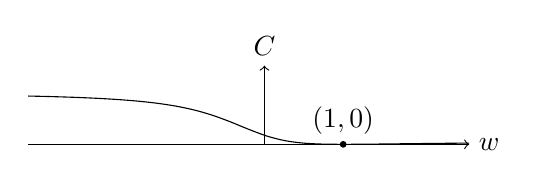
\begin{tikzpicture}
\draw[->] (-3,0) -- (2.6,0) node[right] {$w$};
\draw[->] (0,0) -- (0,1) node[above] {$C$};
\draw[scale=1.0,domain=-3:2.6,smooth,variable=\x,black] plot ({\x},{(((1/(1+e^(-(\x*-3))))-(1/(1+e^(-(-3)))))^2+((1/(1+e^(-(\x*-2))))-(1/(1+e^(-(-2)))))^2+((1/(1+e^(-(\x*-1))))-(1/(1+e^(-(-1)))))^2+((1/(1+e^(-(\x*0))))-(1/(1+e^(-(0)))))^2+((1/(1+e^(-(\x*1))))-(1/(1+e^(-(1)))))^2+((1/(1+e^(-(\x*2))))-(1/(1+e^(-(2)))))^2+((1/(1+e^(-(\x*3))))-(1/(1+e^(-(3)))))^2)/7});
\filldraw[black] (1,0) circle (1pt) node[anchor=south] {$(1,0)$};
\end{tikzpicture}
\caption{A graph of $C$ against $w$}
\label{fig:Cw}
\end{figure}

We know that where $w=1$, we achieve a cost of $0$, so the output is equal to the input. However, we do not want to iterate through all possible weights in a neural network to find the minimum cost, as that is very computationally expensive. Instead, we should start at a random $w$, say $-1$, and take small steps downhill, hence gradient descent. 

\begin{figure}[h]
\setlength{\unitlength}{0.14in}
\centering
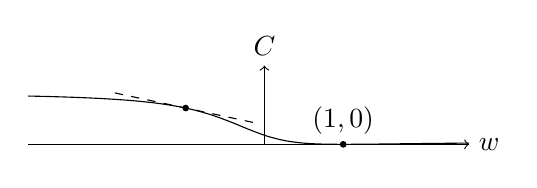
\begin{tikzpicture}
\draw[->] (-3,0) -- (2.6,0) node[right] {$w$};
\draw[->] (0,0) -- (0,1) node[above] {$C$};
\draw[scale=1.0,domain=-3:2.6,smooth,variable=\x,black] plot({\x},{(((1/(1+e^(-(\x*-3))))-(1/(1+e^(-(-3)))))^2+((1/(1+e^(-(\x*-2))))-(1/(1+e^(-(-2)))))^2+((1/(1+e^(-(\x*-1))))-(1/(1+e^(-(-1)))))^2+((1/(1+e^(-(\x*0))))-(1/(1+e^(-(0)))))^2+((1/(1+e^(-(\x*1))))-(1/(1+e^(-(1)))))^2+((1/(1+e^(-(\x*2))))-(1/(1+e^(-(2)))))^2+((1/(1+e^(-(\x*3))))-(1/(1+e^(-(3)))))^2)/7});
\draw[scale=1.0,domain=-1.9:-0.1,dashed,variable=\x,black] plot({\x},{-0.21340427*\x+0.46082-0.21340427});
\filldraw[black] (1,0) circle (1pt) node[anchor=south] {$(1,0)$};
\filldraw[black] (-1,0.46082) circle (1pt);
\end{tikzpicture}
\caption{A graph of $C$ against $w$ showing the gradient at $w=-1$}
\label{fig:Cwm}
\end{figure}
We can decrease the cost, $C$, by repeatedly changing $w$ proportionally to the negative gradient at $w$, or 
\begin{equation}
\Delta w=-\alpha\frac{\partial C}{\partial w}
\end{equation}
where $\alpha$ is the learning rate, which is essentially how big of a step in the given direction you take - too small, and it will take too long finding the minima - too large, and you will overshoot the minima, almost rocking back and forth.

Now, all we need to do is find the gradient.

\subsubsection{Using the Chain Rule}
\label{chain}

Using \fig{fig:XwO}, we can express $C$ as a series of functions 

$$C=(O-Y)^2$$
$$O=\sigma(z)$$
$$z=wX$$

Using the chain rule, we can equate
\begin{equation}
\frac{\partial C}{\partial w}=\frac{\partial C}{\partial O}\frac{\partial O}{\partial z}\frac{\partial z}{\partial w}=2(O-Y)\sigma'(z)X
\label{eq:crw}
\end{equation}
\eq{eq:crw} only works for \fig{fig:XwO}, so we need a more general model. 

Since we are dealing with multiple neurons, weights, and layers, we need a syntax to index these:

$x^L_i$ represents the $i^\text{th}$ neuron in layer $L$;
$Y^L_i$ represents the target for $x^L_i$;
$n_L$ represents the number of neurons in layer $L$;
$w^L_{ij}$ represents the weight of the synapse connected to the $i^\text{th}$ neuron in layer $L$, from the $j^\text{th}$ neuron in layer $L-1$

Consider the following

\begin{figure}[h]
\setlength{\unitlength}{0.14in}
\centering
\begin{picture}(16,5) 

\put(0.8, 0){$\vdots$}
\put(-0.1, 1.6){\framebox(2.2, 2.2){$Y^{L-1}_k$}}
\put(0.8, 4.4){$\vdots$}

\put(3.8, 0){$\vdots$}
\put(2.9, 1.6){\framebox(2.2, 2.2){$x^{L-1}_k$}}
\put(3.8, 4.4){$\vdots$}

\put(11.8, 0){$\vdots$}
\put(10.9, 1.6){\framebox(2.2, 2.2){$x^{L}_j$}}
\put(11.8, 4.4){$\vdots$}

\put(14.8, 0){$\vdots$}
\put(13.9, 1.6){\framebox(2.2, 2.2){$Y^{L}_j$}}
\put(14.8, 4.4){$\vdots$}

\mline{4.5}{0.5}{7.0}{0.0}
\mline{4.5}{0.5}{6.0}{2.15}
\mline{4.5}{0.5}{7.0}{4.3}

\mline{5.5}{2.65}{6.0}{2.15}
\mline{5.5}{2.65}{5.0}{0.0}
\mline{5.5}{2.65}{6.0}{-2.15}

\mline{4.5}{4.8}{7.0}{-4.3}
\mline{4.5}{4.8}{6.0}{-2.15}
\mline{4.5}{4.8}{7.0}{0.0}

\end{picture}
\caption{}
\label{fig:}
\end{figure}
The cost from multiple outputs is the sum of each cost of the output to the corresponding output $$C=\sum_{j=0}^{n_L-1}{(x^L_j-Y_j)^2}$$ The output remains similar to before $$x^L_j=\sigma(z^L_j)$$ where $$z^L_j=\sum_{k=0}^{n_{L-1}-1}w_{jk}^Lx_{k}^{L-1}$$

We can reevaluate the gradient again using the chain rule 

\begin{equation}
\frac{\partial C}{\partial w_{jk}^L}=\frac{\partial C}{\partial x^L_j}\frac{\partial x^L_j}{\partial z^L_j}\frac{\partial z^L_j}{\partial w_{jk}^L}=2(x_{j}^{L}-Y^L_j)\sigma'(z^L_j)x^{L-1}_k
\label{eq:gcrw}
\end{equation}

To find out what $x^{L-1}_k$ should be, $Y^{L-1}_k$, we can use the chain rule against $x^{L-1}_k$ instead of $w_{jk}^L$

\begin{equation}
Y^{L-1}_k=\frac{\partial C}{\partial x^{L-1}_k}=\frac{\partial C}{\partial x^L_j}\frac{\partial x^L_j}{\partial z^L_j}\frac{\partial z^L_j}{\partial x^{L-1}_k}=2(x_{j}^{L}-Y^L_j)\sigma'(z^L_j)w_{jk}^L
\label{eq:gcrY}
\end{equation}

We can then repeat this for each layer going backwards, until all the weights have been rectified to decrease the cost in the most efficient way possible, $\nabla C$. If we repeat this process for each $\{X_i,Y_i\}$ in training set $T$, we would have trained a function to fit to $T$.

\newpage

\section{Methodology}

\subsection{Aim}

Using our knowledge of \gls{model}ling the human brain, learning through the \gls{perceptron} \gls{model}, and back-propagation, we aim to evaluate and justify the extent to which any problem can be taught effectively to a machine such that it is able to give accurate results.

\subsection{Methods}

In order to do this, we must devise a method to measure each of the aspects of a neural network that directly affect the accuracy of the results. Once we have achieved this, we should determine and justify a method for avoiding these aspects for all problems, and then prove it through the use of outlining an optimisation. This should then be met with real-world observations to prove the usefulness of machine learning.

\subsection{Reliability}

The sources I cite are very well known and have been used in academic papers.

\cite{brain} Gordon M. Shepard is a pioneer in the area of neuroscience. He introduced the olfactory system, and used this as a method for \gls{model}ling \gls{dend}s in the brain amongst other areas. His education consists of a MD at Harvard in 1959, and a DPhil at Oxford in 1962. 

“By any measure this work is a classic...It will undoubtedly take its place as one of the most significant and comprehensive commentaries of our time on structure and function of nervous tissue.”--Electrocephalography and Clinical Neurophysiology

\cite{neuron} The experiment consisted of “five elderly men”, and their method produced accurate results.

\cite{hebb} Donald O. Hebb is a psychologist who specialises in understanding human learning. He had recieved 3 honorary doctorates in 1961, 1965, and 1975.

The Organisation of Behavior is seen as Donald Hebb's most affluential piece of work \gls{model}ling our view on neuropsychology.

\cite{learn} “The text is very strong with respect to presenting competing theories of learning phenomena. It is one of the best I’ve read in this regard.”--Thomas J. Faulkenberry

\cite{nnd} “This introductory neural network text targets senior undergraduates, first-year graduate students, and computing professionals who are exploring artificial neural networks.”--Stan J. Thomas


\newpage

\section{Parameters}
\label{params}

\subsection{Learning Paradigms}
\label{paradigms}

A learning paradigm specifies what the general architecture of the \gls{model} is. For example, if we only have inputs to a neural network with no target data, we cannot train a \gls{model} with outputs. As this determines the very core of the design of the \gls{model}, we call this a paradigm.

Consider the different types of learning paradigms, supervised, unsupervised, and reinforcement learning.

\subsubsection{Supervised Learning}

Supervised learning is where the machine is tasked to fit target data. The training set $T$ can be expressed as $$T=\{X_1, Y_1\},\{X_2, Y_2\},\cdots,\{X_I, Y_I\}$$ where $X_i$ is an input, $Y_i$ is the desired outcome of $X_i$, and $I$ is the length of the training set $T$. The machine propagates back through the neural network to adjust the \gls{synapse}s in order to fit closer to the target data.

An example of a supervised learning \gls{model} would be the \gls{perceptron} \gls{model}.

\subsubsection{Unsupervised Learning}

Unsupervised learning is where the machine alters the \gls{synapse}s in the neural network solely based upon the inputs. This is typically used to classify data or cluster data.

An example of an unsupervised \gls{model} is a K-means clustering problem.

\subsubsection{Reinforced Learning}

Reinforcement learning is where the machine is given an environment in which the outputs control, which are then rectified through the environment feedback. For example, if a chess AI made a move, the way we give feedback on the move is through an environment, not target data. 

We can also have a separate neural network act as the environment, in which we call this an adversarial network; the neural network act as each others environment.

\subsection{Determining the Model Parameters}

To determine what \gls{model} parameters we should use, i.e. the number of \gls{hidden} \gls{layer} and \gls{neuron}s in each \gls{layer}, we must understand intuitively what a \gls{neuron} represents and what \gls{layer}s represent.

A \gls{neuron} is a function of the \gls{neuron}s in the previous \gls{layer}. If our function is the product of a training parameter $w$ and a dependent variable $x$, we can treat this as a line $wx$. As we can also train a bias $b$, we result in the equation $wx+b$. If we have multiple \gls{neuron}s in the previous \gls{layer}, we can treat this as a line through multiple dimensions $w_1x_1+w_2x_2+\cdots+b$. In other words, a \gls{neuron} can classify a \gls{lin} relationship from the previous \gls{layer}.

A \gls{layer} can now represent the building and accumulating of features, as if our \gls{lin} relationship takes in \gls{lin} functions, we achieve a \gls{nlin} relationship. As an example, the output should determine the representation of shapes, which classifies the relationship from the previous \gls{layer} of the representation of lines. 

This is to say that if we are able to identify lines in the first \gls{layer}, we can identify lines in those lines in the next \gls{layer}, producing shapes and \gls{nlin} equations. Consider the datasets below

% simple
% o x
% x o


% complex 2-3-2-1
% o x x 
% o o x
% o x x
% o o x

\begin{tikzpicture}
\begin{axis}[%
    scatter/classes={%
        o={mark=o,draw=black},
        x={mark=x,draw=black}
    },
    xlabel={Input 1},
    ylabel={Input 2},
    legend pos=outer north east
]
\addplot[scatter,only marks,%
    scatter src=explicit symbolic]%
table[meta=label] {
x y label
0 0 o
1 0 x
0 1 x
1 1 o
};
\addlegendentry{$0$}
\addlegendentry{$1$}
\end{axis}
\end{tikzpicture}
\hskip 5pt
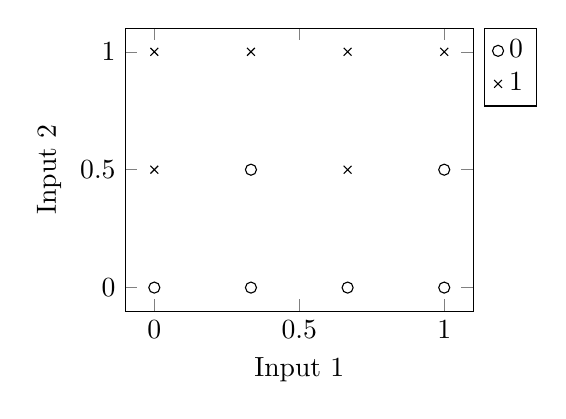
\begin{tikzpicture}
\begin{axis}[%
    scatter/classes={%
        o={mark=o,draw=black},
        x={mark=x,draw=black}
    },
    xlabel={Input 1},
    ylabel={Input 2},
    legend pos=outer north east
]
\addplot[scatter,only marks,%
    scatter src=explicit symbolic]%
table[meta=label] {
x y label
0 0 o
0 0.5 x
0 1 x
0.3333 0 o
0.3333 0.5 o
0.3333 1 x
0.6667 0 o
0.6667 0.5 x
0.6667 1 x
1 0 o
1 0.5 o
1 1 x
};
\addlegendentry{$0$}
\addlegendentry{$1$}
\end{axis}
\end{tikzpicture}

The one on the left can be described as a combination of two lines. As the combination is \gls{lin}, we only need one \gls{layer} for the lines. This gives us the \gls{model} of $2\rightarrow2\rightarrow1$.

The one on the right is more complicated. There are three lines that can be used to classify the different sections in the dataset, but they cannot be combined \gls{lin}ly, as they intersect twice. Therefore, we have the \gls{model} of $2\rightarrow3\rightarrow2\rightarrow1$.

This is backed up by the successfulness of each model architecture for the simple model and complex model in \apdx{resmod}.

\subsection{Determining the Hyperparameters}

The hyperparameters are parameters that you specify before the main computation of the model. This primarily includes the learning rate. The learning rate details how much the weight is changed based on a given gradient. This parameter was discussed earlier in \sect{backprop}, however, it is important to understand how to determine its value.

If your problem is complex, then having too large of a learning parameter could result in your program not finding a solution. This is because it is skipping the points at which the cost is the lowest, and thus we are losing information about the gradient. It can be thought of as though we are randomly trying points until they reach a gradient of 0.

If your problem is simple, then having too small of a learning parameter means that it will take a long time to reach zero cost. This is because when the gradient gets smaller, which will happen with simple examples, the weights change less and less. However, if you use too high of a learning parameter, you risk not finding the shallow gradient, meaning you cycle back and forth between values.


\section{Limitations}
\label{lim}

\subsection{Model Limitations}

\subsubsection{Inaccuracies}
\label{inacc}

If a problem is too complex, the computer may not be able to find a solution. It will therefore resolve a minimum that is equally bad at each input, producing an inaccurate result. This could be due to the simplicity of the model. This decreases the flexibility of the neural network to find patterns. This can be decreased through using a suitable model complexity or giving the machine an incentive to find the correct pattern through the use of \gls{decomposition} and optimisations, or more data such that the pattern is more easily recognised. \cite{ngcan}

\subsubsection{Overfitting}
\label{overfit}

If a neural network has too many parameters or rather more than is needed, it may be able to memorise the input instead of learning a pattern. This gives the illusion that it has worked with the given training data, but when it is given test data, it will not produce accurate results. This is because there are many different solutions to an overly complex model, each with a different pattern. As this cannot, therefore, attribute a single pattern to the model, we do not classify it as learning, but rather memorising. The effect of this can be reduced through simplifying the model to a suitable level or influencing the model to fit to a specific pattern using optimisations and decomposition, or more data such that there is only one pattern that achieves a zero cost.

\subsection{Physical Limitations}

\subsubsection{Data}
\label{limdata}
In supervised learning, you must provide target data to each input. If this data is not sanitised or large enough, the network will find erroneous patterns and produce an incorrect output.\cite{ngcan}

Furthermore, the data you use as input to the neural network must be related to the output, and no relevant data should be left out; the computer doesn't understand the situation, and you cannot assume it does. If you do not know what fields may influence the output, use as much information as possible, increasing only the input \gls{layer} only marginally increases the computation.

This isn't so much of a problem in corporations that manage multiple customers and branches, as they can easily sample data.


\subsubsection{Hardware}

If your model is too complex, especially if it is more complex than it should be, it could take a long time to find a solution. This is because it would have to perform more calculations per \gls{epoch}, and more epochs to find the solution. If you limit the time and computation of training the model, you risk limiting the number of items in your dataset, and you see the same problems that we earlier discussed in \sect{limdata}.

To reduce computation, you can simplify the model, however, if this is not possible, you could implement optimisations and use multiple neural networks that each work on a given simpler task to decompose the problem. 

Again, in large industries, the hardware is abundant, and it usually isn't seen as a limitation.

\subsection{Legal and Ethical Concerns}

There are times when the use of machine learning can produce legal, ethical and moral dilemmas. Concerns include data harvesting, liability, discrimination and profiling, and job displacement. We must take these scenarios into consideration to justify whether a problem can be solved under the law.

\subsubsection{Data Harvesting}

Data Harvesting is where a large corporation surveys and polls information about the clients they serve. This is necessary such that the model that they train will correctly select the targeted advertisement. This has privacy concerns for the client, as some information may be sensitive. The Data Protection Act prohibits companies from storing data about an individual that is not necessarily required for the purpose that the company sells, without their consent. Therefore, companies that do store a lot of information about you, such as Google, require you to consent to their terms. So, although it is legal to use data harvesting, is it moral to have your product only accessible through surrendering your privacy?

\subsubsection{Liability}

Liability is a risk when the output dictates a decision that can have life-threatening consequences. These include autonomous vehicles; if the machine makes a moral decision or mistake, who is responsible? Would it decide to swerve out the way to avoid hurting the group of people, but hurt someone who did nothing wrong or vice versa?

\subsubsection{Discrimination and Profiling}

Profiling is where the machine uses personal information as input to dictate the output. 
This could be dangerous if it determines the opportunity for a service. As an example, if it is used in qualifying loans or credit; is it ethical to use race or gender as inputs when estimating return rates when there is no credit history? It is clear to see that this can cause a discrimination issue.\cite{ngcan}

\subsubsection{Job Displacement}

The most likely threat to our daily lives that machine learning imposes is the use of it in the workforce. Tasks that have a pattern with large amounts of data can be aided significantly with the use of machine learning, decreasing job income and security.

This may not seem to be a large issue as it only affects certain jobs, but when these jobs are likely the entry point for apprenticeships and work experience, the employability for those new to the workforce suffers.

\subsection{Conclusion}

To overcome both model and physical limitations, we require optimisations to decrease computation. The optimisations will have to be specific to the problem itself, as it would otherwise defer from the model we initially have. We could also use decomposition to incentivise the neural network to find more appropriate solutions, where the parts of the total model deal with a simpler problem.



\section{Optimisations}
\label{opt}

We may want our machine to learn more complex problems, where the patterns to learn are more obscure. We could use the \gls{perceptron} \gls{model} and increase the complexity of the model, but this is not very effective as this will drastically increase the computation. Instead we want to find solutions and optimisations to certain types of data that cut down on the number of \gls{neuron}s we use. There are many ways we can optimise for certain types of inputs, but we will look specifically at an unsupervised model, spatial data, and sequential data.

\subsection{Auto-encoders}

Auto-encoders are unsupervised neural networks, as they do not require target data, however, they still have target data to meet. They encode
(compress) the input data into a latent \gls{vec}, $z$, and then decode the latent \gls{vec} into an output that should resemble the input.

\begin{figure}[h]
\setlength{\unitlength}{0.14in}
\centering
\begin{picture}(10, 6) 

\put(0, 0){\framebox(10, 6){}}

\put(4.6, 1.9){\framebox(0.8, 2.2){$z$}}

\mline{0.3}{0.3}{4.0}{1.3}
\mline{0.3}{5.7}{4.0}{-1.3}
\mline{0.3}{0.3}{0.0}{5.4}
\mline{4.3}{1.6}{0.0}{2.8}

\mline{5.7}{4.4}{4.0}{1.3}
\mline{5.7}{1.6}{4.0}{-1.3}
\mline{9.7}{0.3}{0.0}{5.4}
\mline{5.7}{1.6}{0.0}{2.8}

\end{picture}
\caption{Autoencoder block, AE}
\label{fig:aebox}
\end{figure}

\begin{figure}[h]
\setlength{\unitlength}{0.14in}
\centering
\begin{picture}(11,3) 

\put(0.0, 0.6){\framebox(2.2, 2.2){$X_i$}}

\put(4.4, 0.6){\framebox(2.2, 2.2){AE}}

\put(8.8, 0.6){\framebox(2.2, 2.2){$\tilde{X_i}$}}


\mline{2.3}{1.7}{2.0}{0.0}
\mline{6.7}{1.7}{2.0}{0.0}

\end{picture}
\caption{$\tilde{X_i}$ is the decoded output that resembles the input.}
\label{fig:ae}
\end{figure}

If you replace $X_i$ with a function of $X_i$, $f(X_i)$, you can train an inverse function as the auto-encoder.

They train an inverse function $f^{-1}$ from a given function $f$.

$$X=\{X_1,X_2,\cdots,X_I\}$$

There are some common functions that lead to useful outcomes.
Where $f(x) = x$, the auto-encoder acts like a compressor, making it an effective lossy compression
technique to reduce broadband.
Where $f(x)$ is a noise filter, the auto-encoder acts as a denoiser, making it faster to render fragment shaders as you do not have to calculate every pixel.


\begin{figure}[h]
\setlength{\unitlength}{0.14in}
\centering
\begin{picture}(15.4,3) 

\put(0.0, 0.6){\framebox(2.2, 2.2){$X_i$}}

\put(4.4, 0.6){\framebox(2.2, 2.2){$f$}}

\put(8.8, 0.6){\framebox(2.2, 2.2){AE}}

\put(13.2, 0.6){\framebox(2.2, 2.2){$\tilde{X_i}$}}

\mline{2.3}{1.7}{2.0}{0.0}
\mline{6.7}{1.7}{2.0}{0.0}
\mline{11.1}{1.7}{2.0}{0.0}

\end{picture}
\caption{Using a function, we can produce new inputs for our auto-encoder.}
\end{figure}


\begin{figure}[ht]
\setlength{\unitlength}{0.14in}
\centering
\begin{picture}(15.4,3) 

\put(0.0, 0.6){\framebox(2.2, 2.2){$X_i$}}

\put(4.4, 0.6){\framebox(2.2, 2.2){$f$}}

\put(8.8, 0.6){\framebox(2.2, 2.2){$f^{-1}$}}

\put(13.2, 0.6){\framebox(2.2, 2.2){$\tilde{X_i}$}}

\mline{2.3}{1.7}{2.0}{0.0}
\mline{6.7}{1.7}{2.0}{0.0}
\mline{11.1}{1.7}{2.0}{0.0}

\end{picture}
\caption{The auto-encoder then behaves as an inverse of the input function.}
\label{fig:aef}
\end{figure}
\newpage
\subsection{Convolutional Neural Networks}

A convolutional neural network uses a variety of methods to reduce the computation on spatial data, i.e. where the surroundings of the data are important. One method we can use are convolutions, which are \gls{layer}s that find patterns in context of the spatial data easier.\cite[p.~7]{cnn}

This means that the network
requires less \gls{neuron}s, which reduces the risk of overfitting and also saves computation.

\begin{figure}[h]
\setlength{\unitlength}{0.14in}
\centering
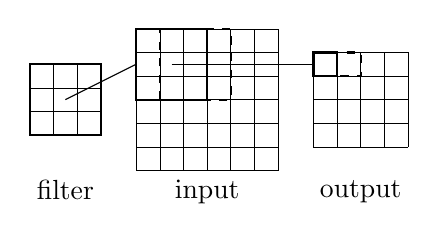
\begin{tikzpicture}[scale=0.30](18,3) 

\node at (1.5, 0) [below] {filter};
\node at (7.5, 0) [below] {input};
\node at (14, 0) [below] {output};

\draw[thick] (0,1.5) rectangle (3, 4.5);
\draw[thick] (12, 4) rectangle (13, 5);
\draw[thick, dashed] (13, 4) rectangle (14, 5);

\draw[thick] (4.5, 3) rectangle (7.5, 6);
\draw[thick, dashed] (5.5, 3) rectangle (8.5, 6);

\draw[step=1, very thin, yshift=0.5cm] (0, 1) grid (3, 4);
\draw[step=1, very thin, xshift=0.5cm] (4, 0) grid (10, 6);
\draw[step=1, very thin] (12, 1) grid (16, 5);

\draw (1.5, 3) -- (4.5, 4.5);
\draw (6, 4.5) -- (12, 4.5);

\end{tikzpicture}
\caption{Output is the convolution of the input given the filter.}
\label{fig:conv}
\end{figure}

The output from a convolution is a \gls{mat} where each node corresponds to the sum of encapsulated nodes multiplied by the filter's respective node.

\begin{equation}
\mx{O}_{ij}=\sum^{1}_{x=-1}{\sum^{1}_{y=-1}{\mx{I}_{(i+x+1)(j+y+1)}\times \mx{F}_{(x+1)(y+1)}}}
\end{equation}

or simply

\begin{equation}
\begin{split}
\mx{O}_{ij}&=\sum^{2}_{x=0}{\sum^{2}_{y=0}{\mx{I}_{(i+x)(j+y)}\times \mx{F}_{xy}}}\\
&=\sum^{X-1}_{x=0}{\sum^{Y-1}_{y=0}{\mx{I}_{(i+x)(j+y)}\times \mx{F}_{xy}}}
\end{split}
\end{equation}

To \gls{bprop} through convolutions, we will use a similar method to what we used in \sect{chain}.

\begin{equation}
\mx{O}=v(\mx{I},\mx{F})
\end{equation}

where $v$ is a function representing a convolution. 


Therefore we can decrease the \gls{cost} $C$, $\nabla C$, using the chain rule for the filter,

\begin{equation}
\begin{split}
\frac{\partial C}{\partial \mx{F}} &= \frac{\partial C}{\partial \mx{O}}\frac{\partial \mx{O}}{\partial \mx{F}}\\
\frac{\partial C}{\partial \mx{F}_{xy}} &= \sum_{i=0}^{I-1}{\sum_{j=0}^{J-1}{\frac{\partial C}{\partial \mx{O}_{ij}}\frac{\partial \mx{O}_{ij}}{\partial \mx{F}_{xy}}}}\\
&= \sum_{i=0}^{I-1}{\sum_{j=0}^{J-1}{\frac{\partial C}{\partial \mx{O}_{ij}}\mx{I-1}_{(i+x)(j+y)}}}\\
\frac{\partial C}{\partial \mx{F}} &=v(\mx{I}, \frac{\partial C}{\partial \mx{O}})
\end{split}
\end{equation}

and also for the image

\begin{equation}
\begin{split}
\frac{\partial C}{\partial \mx{I}} &= \frac{\partial C}{\partial \mx{O}}\frac{\partial \mx{O}}{\partial \mx{I}}\\
\frac{\partial C}{\partial \mx{I}_{ab}} &= \sum_{i=0}^{I-1}{\sum_{j=0}^{J-1}{\frac{\partial C}{\partial \mx{O}_{ij}}\frac{\partial \mx{O}_{ij}}{\partial \mx{I}_{ab}}}}\\
&= \sum_{x=0}^{X-1}{\sum_{y=0}^{Y-1}{\frac{\partial C}{\partial \mx{O}_{(a-x)(b-y)}}\mx{F}_{xy}}}\\
\frac{\partial C}{\partial \mx{I}} &= V(\frac{\partial C}{\partial \mx{O}}, R_{180\degree}\mx{F})
\end{split}
\end{equation}

where $V$ is a full convolution. A full convolution is a convolution that allows for a padding of the output, as $a-x$ or $b-y$ could be outside the range of output.\cite{backcnn}

\begin{figure}[h]
\setlength{\unitlength}{0.14in}
\centering
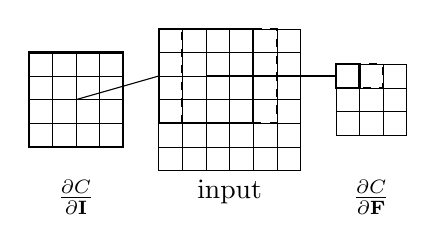
\begin{tikzpicture}[scale=0.30](18,3) 

\node at (2, 0) [below] {$\frac{\partial C}{\partial \mx{I}}$};
\node at (8.5, 0) [below] {input};
\node at (14.5, 0) [below] {$\frac{\partial C}{\partial \mx{F}}$};

\draw[thick] (0,1) rectangle (4, 5);
\draw[thick] (13, 3.5) rectangle (14, 4.5);
\draw[thick, dashed] (14, 3.5) rectangle (15, 4.5);

\draw[thick] (5.5, 2) rectangle (9.5, 6);
\draw[thick, dashed] (6.5, 2) rectangle (10.5, 6);

\draw[step=1, very thin, yshift=0.5cm] (13, 1) grid (16, 4);
\draw[step=1, very thin, xshift=0.5cm] (5, 0) grid (11, 6);
\draw[step=1, very thin] (0, 1) grid (4, 5);

\draw (2, 3) -- (5.5, 4);
\draw (7.5, 4) -- (13, 4);

\end{tikzpicture}
\caption{$\frac{\partial C}{\partial \mx{F}}$ is the output of a convolution with the filter $\frac{\partial C}{\partial \mx{I}}$ on the input.}
\label{fig:filterconv}
\end{figure}

\begin{figure}[h]
\setlength{\unitlength}{0.14in}
\centering
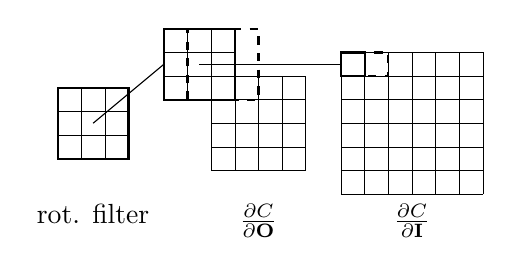
\begin{tikzpicture}[scale=0.30](18,3) 

\node at (1.5, 0) [below] {rot. filter};
\node at (15, 0) [below] {$\frac{\partial C}{\partial \mx{I}}$};
\node at (8.5, 0) [below] {$\frac{\partial C}{\partial \mx{O}}$};

\draw[thick] (0,1.5) rectangle (3, 4.5);
\draw[thick] (12, 5) rectangle (13, 6);
\draw[thick, dashed] (13, 5) rectangle (14, 6);

\draw[thick] (4.5, 4) rectangle (7.5, 7);
\draw[thick, dashed] (5.5, 4) rectangle (8.5, 7);

\draw[step=1, very thin, xshift=0.5cm] (4, 4) grid (7, 7);
\draw[step=1, very thin, yshift=0.5cm] (0, 1) grid (3, 4);
\draw[step=1, very thin] (12, 0) grid (18, 6);
\draw[step=1, very thin, xshift=0.5cm] (6, 1) grid (10, 5);

\draw (1.5, 3) -- (4.5, 5.5);
\draw (6, 5.5) -- (12, 5.5);

\end{tikzpicture}
\caption{$\frac{\partial C}{\partial \mx{I}}$ is the output of the full convolution $\frac{\partial C}{\partial \mx{O}}$ given a filter rotated by 180\degree}
\label{fig:fullconv}
\end{figure}

By using multiple convolutional \gls{layer}s in series, you teach the neural network to decompose features of the images, such as lines and shapes, which helps a feed-forward neural network to decrease the \gls{cost}. For example, the first \gls{layer} may pick out edges, the next lines, and then shapes.

We can also use pooling, which is a method of finding only the important information. It works similarly to a convolution, except the filter is constant, and uses a function instead of a summation, such as returning the maximum. This helps condense the output from convolutions.

In conclusion, we can use convolutions and pooling to help and optimise feed-forward networks to find patterns in spatial data. This is because the trainable parameters are only concerned in data surrounding a node. 

Moreover, this concludes that if we can differentiate a function to propagate forward and calculate a \gls{cost}, we are able to adjust the parameters of the function to decrease the \gls{cost}. 

\subsection{Recurrent Neural Networks}
\label{recurrent}

Recurrent neural networks are supervised neural networks that allow you to analyse sequential data. They work by feeding the current state into itself, which allows you to predict states of a system in the future based on the present.

\begin{figure}[ht]
\setlength{\unitlength}{0.14in}
\centering
\begin{picture}(10,7.2) 

\put(0.0, 0.6){\framebox(2.2, 2.2){$X$}}

\put(4.4, 0.6){\framebox(2.2, 2.2){$h$}}

\put(8.8, 0.6){\framebox(2.2, 2.2){$y$}}

\mline{2.3}{1.7}{2.0}{0.0}
\mline{6.7}{1.7}{2.0}{0.0}


\put(0.0, 5){\framebox(2.2, 2.2){$X$}}

\put(4.4, 5){\framebox(2.2, 2.2){$h$}}

\put(8.8, 5){\framebox(2.2, 2.2){$y$}}

\mline{2.3}{6.1}{2.0}{0.0}
\mline{6.7}{6.1}{2.0}{0.0}

\mline{5.4}{2.9}{0.0}{2.0}

\end{picture}
\caption{A recurrent neural network feeding the present state into the next.}
\label{fig:rnn}
\end{figure}

Back-propagating through this architecture is quite complex. It requires you to back-propagate through each state, which therefore implies that the more states you have, the more operations you would have to do. You would also have to store each of the inputs and outputs for each state.\cite{rnn}

Aside from this minor difference, the algebra of back-propagation is the same.



\section{Modelling Optimisations}


Now that we have seen how to \gls{model} a neural network such that the machine can perform gradient descent on relevant data, we can create our own \gls{model}s.

\subsection{Variational Auto-encoder}

A variational auto-encoder attempts to use a latent \gls{vec}, $z$, that is a sample from a probability distribution of a variable. Therefore, the encoder, $q_\phi(z|X)$ must be a distribution. As a probability distribution is defined as $N(\mu, \sigma^2)$, we can sample the latent \gls{vec} from a mean \gls{vec} and a standard deviation \gls{vec}.  

\begin{figure}[ht]
\setlength{\unitlength}{0.14in}
\centering
\begin{picture}(26.4,8) 
\put(0, 2.0){\framebox(2.2, 2.2){$X$}}

\mline{2.7}{5.6}{5.0}{-2.8}
\mline{2.7}{0.6}{5.0}{0.0}
\mline{7.7}{0.6}{0.0}{2.2}
\mline{2.7}{0.6}{5.0}{2.8}
\mline{2.7}{5.6}{5.0}{0.0}
\mline{2.7}{0.6}{0.0}{5.0}
\mline{7.7}{3.4}{0.0}{2.2}

\put(8.2, 3.4){\framebox(2.2, 2.2){$\mu$}}

\put(8.2, 0.6){\framebox(2.2, 2.2){$\sigma$}}

\put(2.1, 6.1){$\overbrace{\qquad\qquad\qquad\qquad\quad}^{q_\phi(z|X)}$}

\put(10.9, 2.9){$\left\} \rule{0pt}{12mm}\right.$}

\put(12.6, 2.0){\framebox(2.2, 2.2){$z$}}

\mline{15.3}{2.0}{5.0}{-1.4}
\mline{15.3}{4.2}{5.0}{1.4}
\mline{20.3}{0.6}{0.0}{5.0}
\mline{15.3}{2.0}{0.0}{2.2}

\put(11.9, 6.1){$\overbrace{\qquad\qquad\qquad\qquad\quad}^{p_\theta(\tilde{X}|z)}$}

\put(20.8, 2.0){\framebox(2.2, 2.2){$\tilde{X}$}}

\end{picture}
\caption{The varaitional auto-encoder with the probabilistic encoder $q_\phi$ and decoder $p_\theta$.}
\label{fig:vae}
\end{figure}

Sampling from a distribution allows the variable to represent a feature, as small changes in a feature should have a similar output. However, since this give a greater reconstruction loss than a regular auto-encoder due to the restriction, the standard deviation, $\sigma$, will become $0$, such that it acts as a regular auto-encoder. Therefore, we must compare the sample distribution, $N(\mu, \sigma^2)$, to a distribution of $\sigma=1$, $N(0,1)$, and make sure they are roughly equal. This function is called the Kullback–Leibler divergence, $D_{KL}(\alpha||\beta)$, and returns $0$ when the distributions $\alpha,\beta$ are equal.

As we cannot back-\gls{prop} through a sample of a distribution, we have to take out the sampled distribution into a normal variable, and then apply the standard deviation and mean to achieve a result. This will then give us a method of back-propagating through the variables. This essentially gives us $z=\sigma x+\mu$, where $x\sim N(0,1)$.


\section{Uses of Machine Learning}

\subsection{Present Uses}

With growing data sets and dispensable hardware, machine learning is becoming increasingly more relevant in today's industry. Primary focuses are on detecting patterns in user's search history for advertisement, face recognition for social media sites, commuting predictions for traffic, surveillance footage for reporting crimes, and translation from and to different languages.
Any laborious and extensive task that seems simple can probably be and is automated using machine learning.

“It is difficult to think of a major industry that AI will not transform. This includes healthcare, education, transportation, retail, communications, and agriculture. There are surprisingly clear paths for AI to make a big difference in all of these industries.”--Andrew Ng

\subsection{Future Uses}

Machine learning has already in place for simple tasks for decades, however, only recently has hardware become so cheap and accessible that we can now use machine learning to accelerate complex algorithms such as fluid simulation, where the output doesn't have to be exactly accurate, as long as it is reasonable to the human eye. Another example would be in DLSS for ray trace rendering. It samples some of the rays to produce a low-quality noisy image, passes it through a network and produces a high-quality image.

Recently, there has been a scientific breakthrough in the field of biological engineering due to advancements in machine learning. Google's DeepMind software “AlphaFold 2”, has been able to accurately predict the folding of protein structures, a problem that has been around for 50 years. Researchers believe it will enable us to understand viruses, create drugs, and design vaccines. 

\newpage


\section{Conclusion}
\label{conc}

\subsection{Summary}

We have seen the correlation between machine learning and human learning, \gls{model}ling learning through the \gls{perceptron}, understanding how learning occurs through back-propagation, and how we can expand this knowledge to create specific architectures and \gls{model}s.

With these ideas, we were able to find limitations to given problems, and what is required for a machine to learn. Once we have arrived at a clear \gls{model} for solving problems, we then discussed the ethics and legality of doing so.

\subsection{Main Conclusion}

It is clear to see that with a \gls{model} that does not have any assumptions, enough data, and a \gls{model} complexity that mirrors the complexity of the problem, we can teach a machine any problem through \gls{decomposition} and our own understanding, to influence the machine to learn a pattern.

It should therefore be considered if it is legal or ethically possible, which under certain conditions, produces moral concerns.

\subsection{Recommendations for Further Work}

There are numerous areas where further research was necessary to produce a clear argument for how more complex architectures are designed and used. This includes researching and designing different activations, different methods of back-propagation, and complex problems that require decomposition and \gls{decomposition} of multiple neural architectures.



\addcontentsline{toc}{section}{References}
\bibliographystyle{unsrt}
\bibliography{bibliography}

\newpage

\appendix

\printglossary



\section{Results}
\label{results}
\subsection{Gradient Descent}
\label{resgd}
\begin{figure}[H]
\centering
\includegraphics[width=14cm]{images/gradientdescent2.png}
\caption{We can see from our own example, that the cost is being reduced in the most efficient way, $\nabla C$ by adjusting the weights.}
\end{figure}

\subsection{Training Model}
\label{restm}
\begin{figure}[H]
\includegraphics[width=7cm]{images/1.png}
\includegraphics[width=7cm]{images/2.png}
\includegraphics[width=7cm]{images/3.png}
\includegraphics[width=7cm]{images/4.png}
\caption{The data the model uses is an XOR function. With each epoch iteration of 750, we can see how our function (fit) gets closer to the actual results (data), decreasing the cost.}
\end{figure}

\subsection{Model Parameters}
\label{resmod}

\subsubsection{Simple Model}
\label{ressimp}
\begin{figure}[H]

\includegraphics[width=4.6cm]{images/parameters/simple/line-.png}
\includegraphics[width=4.6cm]{images/parameters/simple/line.png}
\includegraphics[width=4.6cm]{images/parameters/simple/line+.png}

\caption{Left model: 2-1; Middle model: 2-2-1; Right model: 2-3-2-1;}
\end{figure}

\subsubsection{Complex Model}
\label{rescomp}
\begin{figure}[H]

\includegraphics[width=4.6cm]{images/parameters/complex/line-.png}
\includegraphics[width=4.6cm]{images/parameters/complex/line.png}
\includegraphics[width=4.6cm]{images/parameters/complex/line+.png}

\caption{Left model: 2-2-1; Middle model: 2-3-2-1; Right model: 2-8-4-2-1;}
\end{figure}

The left model of 2-2-1 results in a cost of approximately zero. There are many reasons that could allow this to happen. Firstly, two hidden neurons implies that there are two linear lines, however, that is clearly not possible given the data. Therefore there must be a type of rounding error that allows more complexity in the neuron. Secondly, since we are using a sigmoid activation function, it limits the range to $0<x<1$. Therefore, the combination of these lines do not have to be non-linear, as our activation is not.

\end{document}
